\documentclass[ngerman, a4paper, 11pt]{scrartcl}

\usepackage[top=2.5cm,bottom=2.5cm,left=2.5cm,right=2.5cm]{geometry}
\usepackage{parskip}
\usepackage[onehalfspacing]{setspace} % increase row-space

\usepackage[ngerman]{babel}
\usepackage[utf8]{inputenc}
\usepackage{lmodern}
\usepackage[scale=0.8]{opensans}
\newcommand*{\osfamily}{\fontfamily{fos}\selectfont}
\DeclareTextFontCommand{\textos}{\osfamily}
\usepackage{bold-extra}

\usepackage[normalem]{ulem}
\usepackage[autostyle=true,english=british]{csquotes}
\usepackage{enumerate}
\usepackage[inline]{enumitem} % customize label
\usepackage{graphicx}
\usepackage[table,dvipsnames]{tudscrcolor} % package xcolor loaded automatically
\usepackage[font=small,labelfont=bf]{caption} % captions of non-floated figures

\usepackage{listings}
\lstset{ 
	backgroundcolor=\color{cdgray!5},   
	basicstyle=\small\ttfamily,        
	breakatwhitespace=false,         
	breaklines=true,                 
	captionpos=b,                    
	commentstyle=\color{gray},    
	escapeinside={\%*}{*)},         
	extendedchars=true,              
	firstnumber=1,               
	frame=single,	                   
	keepspaces=true,                 
	%keywordstyle=\bfseries\color{blue},      
	language=C,                
	morekeywords={*,...},            
	numbers=none,                    
	numbersep=5pt,                   
	%numberstyle=\tiny\color{mygray}, 
	rulecolor=\color{black},         
	showspaces=false,                
	showstringspaces=false,          
	showtabs=false,                  
	stepnumber=2,                    
	%stringstyle=\color{mymauve},
	tabsize=4,	                              
}

\usepackage[
	type={CC},
	modifier={by-nc-sa},
	version={4.0},
]{doclicense}

\usepackage[unicode,bookmarks=true]{hyperref}
\hypersetup{
	colorlinks,
	urlcolor=cdblue,
	pdfborder={0 0 0}			% no boxed around links
	pdfborderstyle={/S/U/W 1},	% underlining insteas of boxes
	linkbordercolor=cdblue,
	urlbordercolor=cdblue
}

\newcommand*\ruleline[1]{\par\noindent\raisebox{.8ex}{\makebox[\linewidth]{\hrulefill\hspace{1ex}\raisebox{-.8ex}{#1}\hspace{1ex}\hrulefill}}}


\begin{document}

\begin{center}
	{\bfseries \sffamily \huge Wieso brauchen wir Doppelreferenzen?} 
	
	\ruleline{\sffamily \Large Übungsblatt 6}
	
	{\scshape Eric Kunze --- \today}
\end{center}
\medskip

{ \footnotesize \doclicenseThis }

\begin{center}
	\small 
	Die Ausführungen basieren auf einem OPAL-Forum-Post aus dem Wintersemester 2020/21, siehe \url{https://bildungsportal.sachsen.de/opal/auth/RepositoryEntry/26663256067/CourseNode/101767297876002/Message/29317267462}.
	
	\slshape Keine Garantie auf Vollständigkeit und/oder Korrektheit!
\end{center}

\bigskip

Wir betrachten eine einfach-verkettete Liste, definiert durch folgenden Datentyp:
\begin{lstlisting}
typedef struct element *list;
struct element {
	int value;
	list next;
};
\end{lstlisting}

Wir wollen nun beispielhaft das Anhängen an das Ende der Liste ansehen. Dazu sei zunächst eine einfache Hilfsfunktion zum Ausgeben einer Liste gegeben:
\begin{lstlisting}
void print(list lp) {
	printf("[");
	
	while(lp != NULL) {
		printf("%d, ", lp->value);
		lp = lp->next;
	}
	
	printf("]\n");
}
\end{lstlisting}

Man beachte dabei, dass dieses \lstinline[]|print| nichts mit der \enquote{Standard-Ausgabe} \lstinline[]|printf| zu tun hat und insbesondere nicht standardmäßig implementiert ist.


\section{Einfache Referenzen}

Wir versuchen zunächst dieses Problem mit einfachen Referenzen zu lösen, d.h. der Kopf unserer Funktion soll so aussehen: \lstinline[]|void append_p(list lp, int n)|.

\begin{center}
	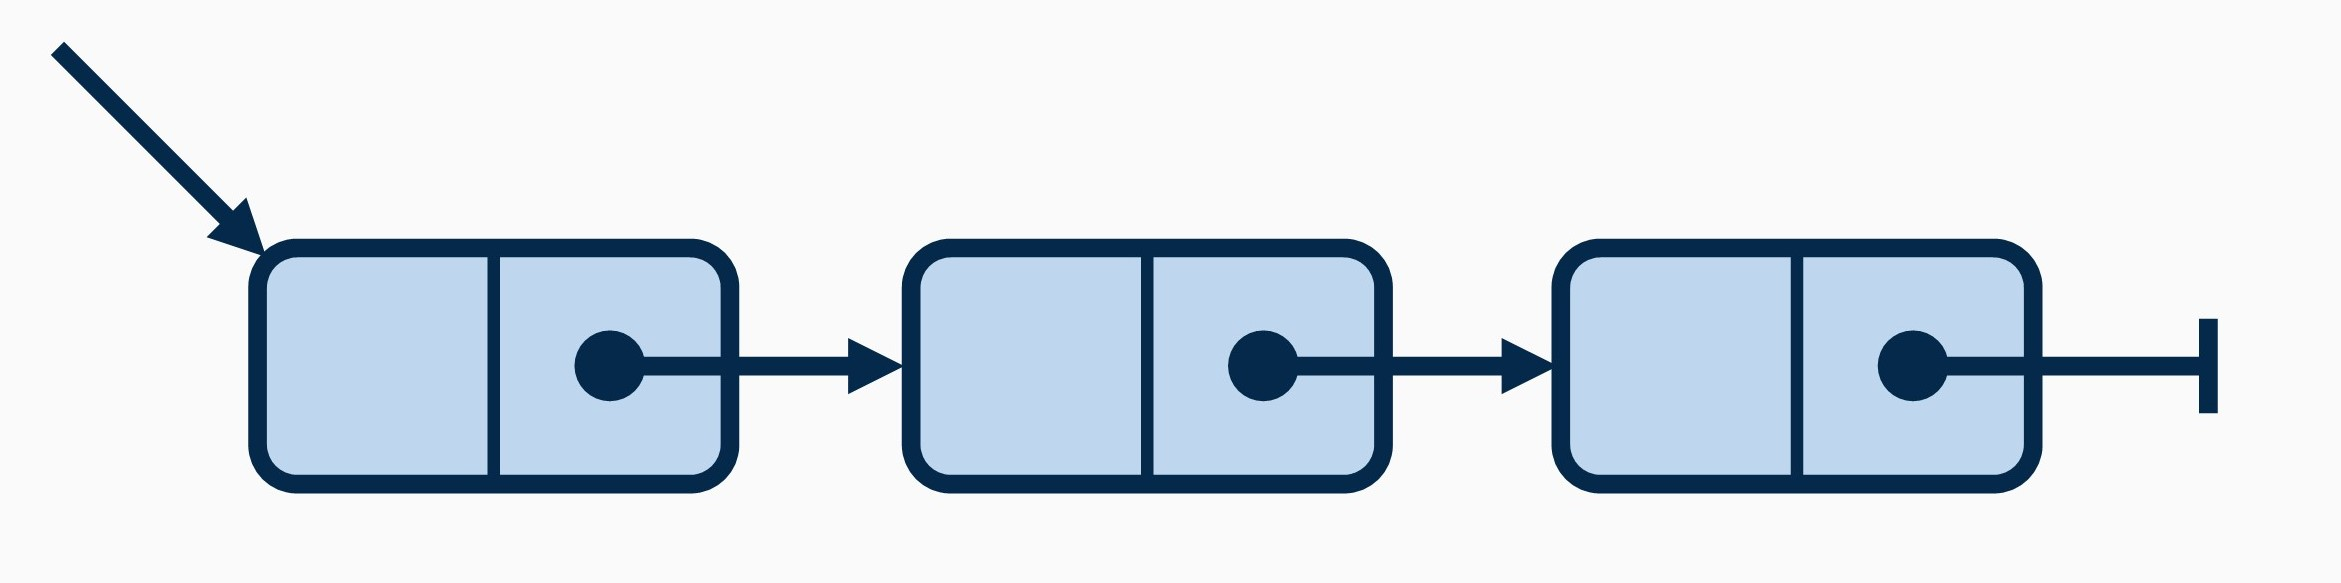
\includegraphics[width=0.5\linewidth]{./tut06-graphics/tut06_einfacheReferenz.jpg}
\end{center}


Zunächst gehen wir bis zum Ende der Liste, indem wir in einer \texttt{while}-Schleife den Pointer immer weiter setzen bis wir schließlich den \texttt{NULL}-Pointer am Ende erreichen. Dann können wir mit \texttt{malloc} ein neues \texttt{struct element} erzeugen, dieses entsprechend befüllen und abschließend die Verknüpfung zur bisherigen Liste herstellen.
\begin{lstlisting}
void append_p(list lp, int n) {
	while(lp->next != NULL)
		lp = lp->next;
	
	struct element *c = malloc(sizeof(struct element));
	c->value = n;
	c->next = NULL;
	
	lp->next = c;
}
\end{lstlisting}

Testen wir diese Funktion mithilfe der folgenden \texttt{main}:
\begin{lstlisting}
int main(void) {
	list l = malloc(sizeof *l);
	l->value = 2;
	l->next = NULL;
	
	append_p(l, 4);
	print(l);
}
\end{lstlisting}
so erhalten wir die Ausgabe \texttt{[2, 4]}; es scheint also alles geklappt zu haben. 
Nun kommen wir aber zum Problemfall: was passiert, wenn unsere Liste nicht initial mit einer \texttt{2} gefüllt ist, sonder initial leer ist?
\begin{lstlisting}
int main(void) {
	list l = NULL;
	
	append_p(l, 4);
	append_p(l, 2);
	
	print(l);
}
\end{lstlisting}
Dieses Programm wird nicht wie erhofft funktionieren, da wir in der \lstinline{append_p}-Funktion versuchen, einen \texttt{NULL-Pointer} zu derefenzieren, wenn wir die Schleifenbedingung \lstinline|lp->next != NULL| prüfen. Genauer entsteht ein zufälliger Speicherzugriff; ein \enquote{segmentation fault} oder \enquote{access violation}.


\section{Ein Ausweg mit einfachen Referenzen?}

Nun versucht man natürlich erst einmal mit einfachen Mitteln (d.h. einfachen Referenzen) auch den Fall der leeren Liste einzubeziehen. Dabei könnte folgende Funktion entstehen:
\begin{lstlisting}
void append_p(list lp, int n) {
	while(lp != NULL)
		lp = lp->next;
	
	lp = malloc(sizeof(struct element));
	lp->value = n;
	lp->next = NULL;
}
\end{lstlisting}

Damit wird der \texttt{NULL}-Pointer nicht mehr dereferenziert, sondern direkt geprüft (\textit{ohne} Dereferenzierung in der Schleifenbedingung). Nun bekommt man allerdings ein neues Problem. Nutzen wir obige \texttt{main}-Funktion, so erhalten wir die Ausgabe \texttt{[]} --- ein merkwürdiges Verhalten, das sich aber mithilfe des pulsierenden Speichers erklären lässt. Beim Aufruf von \lstinline[]|append_p(l, 4)| wird der Pointer \texttt{l} \textit{kopiert} und in \texttt{lp} gespeichert. Ändert man nun innerhalb von \lstinline[]|append_p| den \texttt{lp}-Pointer, so ändert sich der \texttt{l}-Pointer in der \texttt{main}-Funktion \textit{nicht}. Beim Rücksprung geht \texttt{lp} dann vollständig verloren, der bearbeitete Speicher ist nicht mehr erreichbar und wir halten nur noch den unveränderten \texttt{l}-Pointer der \texttt{main}. Somit gilt auch nach den beiden Aufrufen \lstinline[]|append_p(l, 4)| und \lstinline[]|append_p(l, 2)| noch \lstinline{l == NULL} und eine leere Liste wird ausgegeben.

Somit ist dieser \enquote{Ausweg} mit einfachen Referenzen offensichtlich nicht zielführend.


\section{Ausweg: doppelte Referenzen}

\begin{center}
	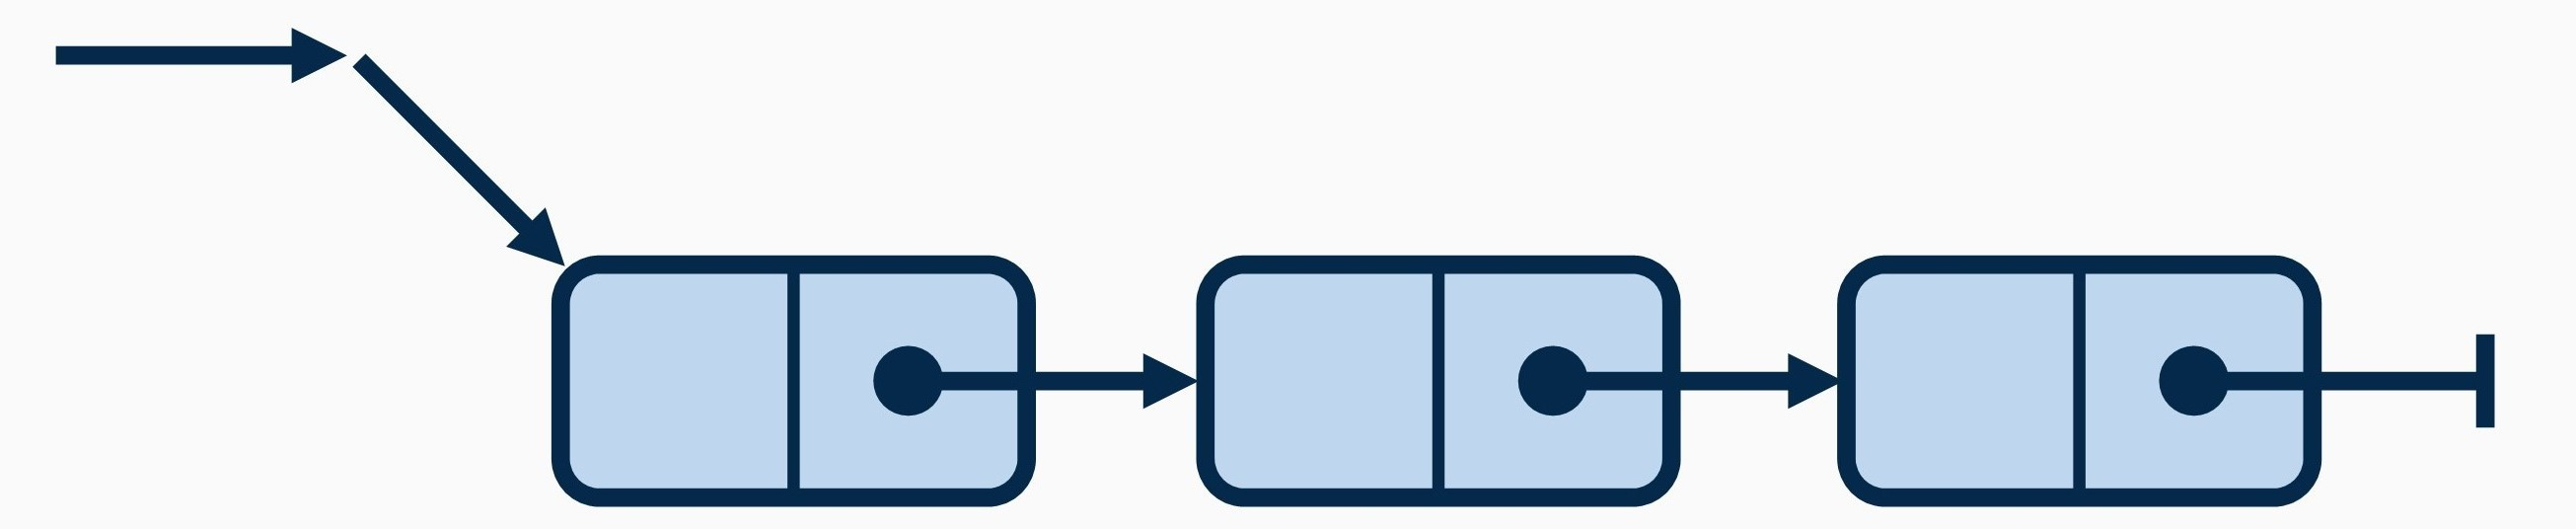
\includegraphics[width=0.75\linewidth]{./tut06-graphics/tut06_doppelReferenz.jpg}
\end{center}

Nun zeigen wir abschließend noch eine funktionierende Variante, die auch leere Listen behandeln kann und ihre Arbeit beim Rücksprung nicht verwirft.
Dies erreichen wir, indem beim Funktionsaufruf nicht eine Kopie des Pointers übergeben wird, sondern wiederum eine Referenz auf den Pointer (so entsteht eine Doppelreferenz). Damit manipulieren wir innerhalb der \lstinline[]|append_pp|-Funktion die originalen Pointer und Daten und nicht eine Kopie davon.

\pagebreak

\begin{lstlisting}
void append_pp(list *lp, int n) {
	while(*lp != NULL)
		lp = &(*lp)->next;
	
	struct element *c = malloc(sizeof(struct element));
	c->value = n;
	c->next = NULL;
	
	*lp = c;
}
\end{lstlisting}

Mit der zugehörigen \texttt{main}
\begin{lstlisting}
int main(void) {
	list l = NULL;
	
	append_pp(&l, 4);
	append_pp(&l, 2);
	
	print(l);
}
\end{lstlisting}
erhalten wir schließlich die erhoffte Ausgabe \texttt{[2, 4, ]}.

\end{document}
